% Generated from figures/generated/sequence.svg; do not hand edit.
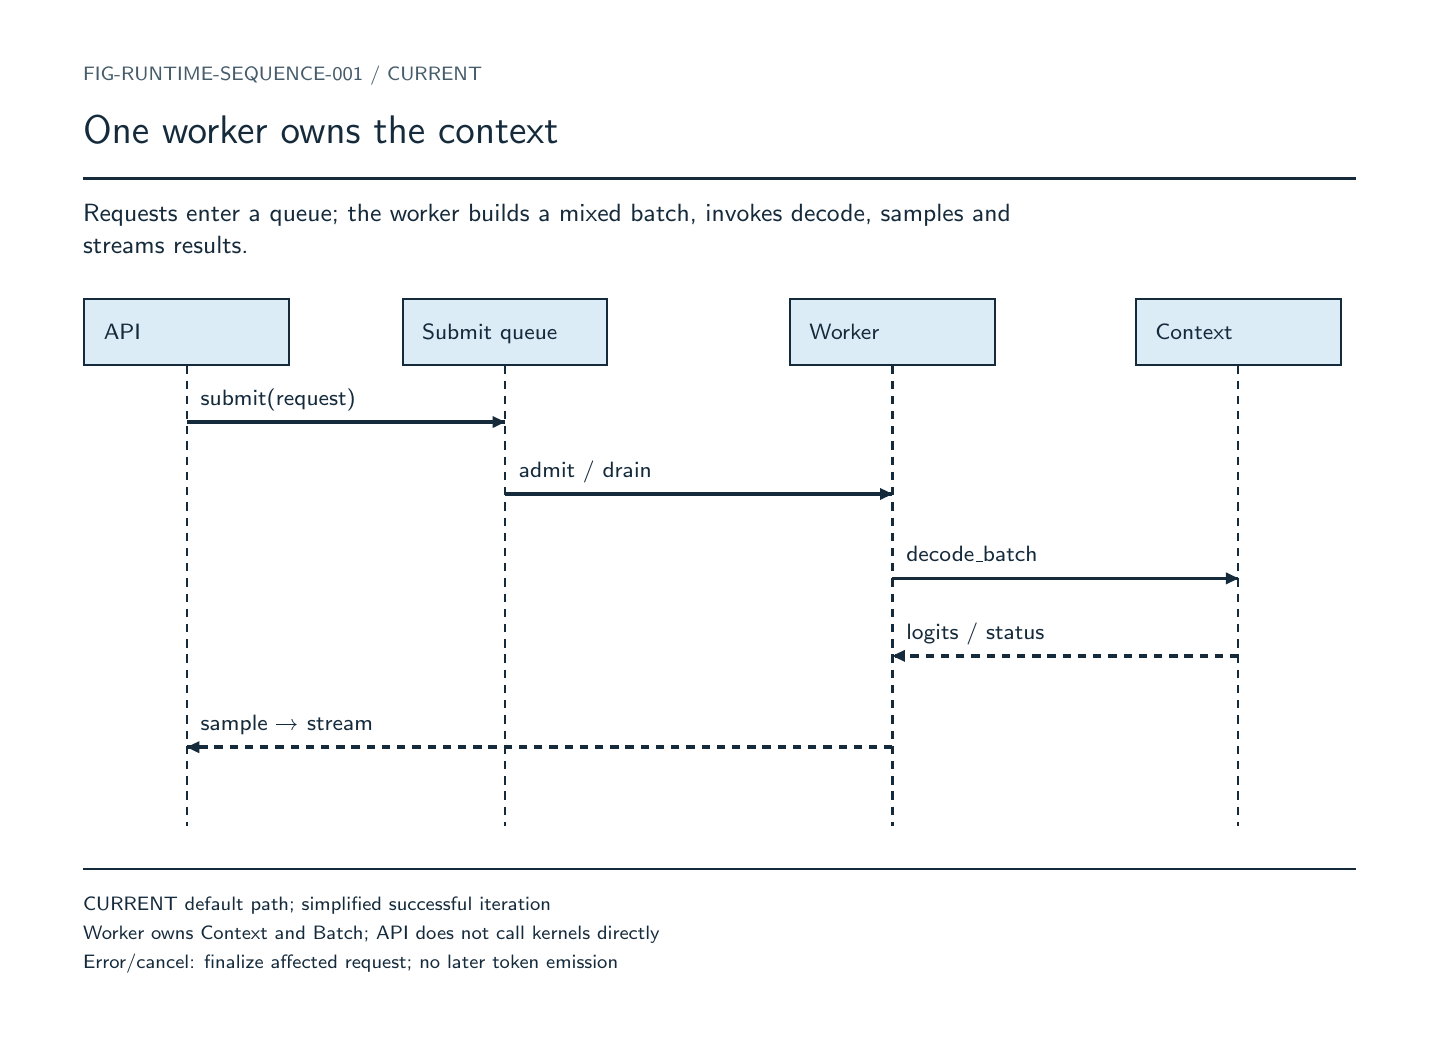
\begin{tikzpicture}[x=.5pt,y=-.5pt]
\path[use as bounding box] (0,0) rectangle (1000,720);
\path[fill=white,draw=none,line width=0.5pt] (0.0,0.0) rectangle (1000.0,720.0);
\node[inner sep=0pt,outer sep=0pt,anchor=base west,text={rgb,255:red,70;green,92;blue,107},font=\sffamily\fontsize{7.0}{8.4}\selectfont] at (40,38) {FIG-RUNTIME-SEQUENCE-001  /  CURRENT};
\node[inner sep=0pt,outer sep=0pt,anchor=base west,text={rgb,255:red,21;green,43;blue,60},font=\sffamily\fontsize{15.0}{18.0}\selectfont] at (40,84) {One worker owns the context};
\draw[fill=none,draw={rgb,255:red,21;green,43;blue,60},line width=0.75pt] (40,109) -- (960,109);
\node[inner sep=0pt,outer sep=0pt,anchor=base west,text={rgb,255:red,21;green,43;blue,60},font=\sffamily\fontsize{9.5}{11.4}\selectfont] at (40,140) {Requests enter a queue; the worker builds a mixed batch, invokes decode, samples and};
\node[inner sep=0pt,outer sep=0pt,anchor=base west,text={rgb,255:red,21;green,43;blue,60},font=\sffamily\fontsize{9.5}{11.4}\selectfont] at (40,163) {streams results.};
\path[fill={rgb,255:red,220;green,236;blue,247},draw={rgb,255:red,21;green,43;blue,60},line width=0.7pt] (41.0,196.0) rectangle (189.0,244.0);
\node[inner sep=0pt,outer sep=0pt,anchor=base west,text={rgb,255:red,21;green,43;blue,60},font=\sffamily\fontsize{8.5}{10.2}\selectfont] at (55,225) {API};
\draw[fill=none,draw={rgb,255:red,21;green,43;blue,60},line width=0.75pt,dash pattern=on 3.0pt off 2.5pt] (115,244) -- (115,577);
\path[fill={rgb,255:red,220;green,236;blue,247},draw={rgb,255:red,21;green,43;blue,60},line width=0.7pt] (271.0,196.0) rectangle (419.0,244.0);
\node[inner sep=0pt,outer sep=0pt,anchor=base west,text={rgb,255:red,21;green,43;blue,60},font=\sffamily\fontsize{8.5}{10.2}\selectfont] at (285,225) {Submit queue};
\draw[fill=none,draw={rgb,255:red,21;green,43;blue,60},line width=0.75pt,dash pattern=on 3.0pt off 2.5pt] (345,244) -- (345,577);
\path[fill={rgb,255:red,220;green,236;blue,247},draw={rgb,255:red,21;green,43;blue,60},line width=0.7pt] (551.0,196.0) rectangle (699.0,244.0);
\node[inner sep=0pt,outer sep=0pt,anchor=base west,text={rgb,255:red,21;green,43;blue,60},font=\sffamily\fontsize{8.5}{10.2}\selectfont] at (565,225) {Worker};
\draw[fill=none,draw={rgb,255:red,21;green,43;blue,60},line width=0.75pt,dash pattern=on 3.0pt off 2.5pt] (625,244) -- (625,577);
\path[fill={rgb,255:red,220;green,236;blue,247},draw={rgb,255:red,21;green,43;blue,60},line width=0.7pt] (801.0,196.0) rectangle (949.0,244.0);
\node[inner sep=0pt,outer sep=0pt,anchor=base west,text={rgb,255:red,21;green,43;blue,60},font=\sffamily\fontsize{8.5}{10.2}\selectfont] at (815,225) {Context};
\draw[fill=none,draw={rgb,255:red,21;green,43;blue,60},line width=0.75pt,dash pattern=on 3.0pt off 2.5pt] (875,244) -- (875,577);
\draw[fill=none,draw={rgb,255:red,21;green,43;blue,60},line width=1.25pt] (115,285) -- (345,285);
\path[fill={rgb,255:red,21;green,43;blue,60},draw=none,line width=0.5pt] (345.00,285.00) -- (336.00,289.35) -- (336.00,280.65) -- cycle;
\node[inner sep=0pt,outer sep=0pt,anchor=base west,text={rgb,255:red,21;green,43;blue,60},font=\sffamily\fontsize{8.5}{10.2}\selectfont] at (125,273) {submit(request)};
\draw[fill=none,draw={rgb,255:red,21;green,43;blue,60},line width=1.25pt] (345,337) -- (625,337);
\path[fill={rgb,255:red,21;green,43;blue,60},draw=none,line width=0.5pt] (625.00,337.00) -- (616.00,341.35) -- (616.00,332.65) -- cycle;
\node[inner sep=0pt,outer sep=0pt,anchor=base west,text={rgb,255:red,21;green,43;blue,60},font=\sffamily\fontsize{8.5}{10.2}\selectfont] at (355,325) {admit / drain};
\draw[fill=none,draw={rgb,255:red,21;green,43;blue,60},line width=1.25pt] (625,398) -- (875,398);
\path[fill={rgb,255:red,21;green,43;blue,60},draw=none,line width=0.5pt] (875.00,398.00) -- (866.00,402.35) -- (866.00,393.65) -- cycle;
\node[inner sep=0pt,outer sep=0pt,anchor=base west,text={rgb,255:red,21;green,43;blue,60},font=\sffamily\fontsize{8.5}{10.2}\selectfont] at (635,386) {decode\_batch};
\draw[fill=none,draw={rgb,255:red,21;green,43;blue,60},line width=1.25pt,dash pattern=on 3.0pt off 2.5pt] (875,454) -- (625,454);
\path[fill={rgb,255:red,21;green,43;blue,60},draw=none,line width=0.5pt] (625.00,454.00) -- (634.00,449.65) -- (634.00,458.35) -- cycle;
\node[inner sep=0pt,outer sep=0pt,anchor=base west,text={rgb,255:red,21;green,43;blue,60},font=\sffamily\fontsize{8.5}{10.2}\selectfont] at (635,442) {logits / status};
\draw[fill=none,draw={rgb,255:red,21;green,43;blue,60},line width=1.25pt,dash pattern=on 3.0pt off 2.5pt] (625,520) -- (115,520);
\path[fill={rgb,255:red,21;green,43;blue,60},draw=none,line width=0.5pt] (115.00,520.00) -- (124.00,515.65) -- (124.00,524.35) -- cycle;
\node[inner sep=0pt,outer sep=0pt,anchor=base west,text={rgb,255:red,21;green,43;blue,60},font=\sffamily\fontsize{8.5}{10.2}\selectfont] at (125,508) {sample → stream};
\draw[fill=none,draw={rgb,255:red,21;green,43;blue,60},line width=0.75pt] (40,608) -- (960,608);
\node[inner sep=0pt,outer sep=0pt,anchor=base west,text={rgb,255:red,21;green,43;blue,60},font=\sffamily\fontsize{7.5}{9.0}\selectfont] at (40,638) {CURRENT default path; simplified successful iteration};
\node[inner sep=0pt,outer sep=0pt,anchor=base west,text={rgb,255:red,21;green,43;blue,60},font=\sffamily\fontsize{7.5}{9.0}\selectfont] at (40,659) {Worker owns Context and Batch; API does not call kernels directly};
\node[inner sep=0pt,outer sep=0pt,anchor=base west,text={rgb,255:red,21;green,43;blue,60},font=\sffamily\fontsize{7.5}{9.0}\selectfont] at (40,680) {Error/cancel: finalize affected request; no later token emission};
\end{tikzpicture}
